\chapter{Proof of Stake}
\section{Proof of Work is energy inefficient}
The blockchains we have seen this far, from Bitcoin to its improvements, are based on the proof of work (PoW) mining procedure.\\
The design depends on the PoW process, which has several functions: it prevents spam on the network, it elects block proposers, and it protects against Sybil attacks on the protocol.\\\\
However, PoW mining is very wasteful of energy and hardware resources (GPUs). It has been estimated that Bitcoin’s electricity consumption is similar to that of a mid-sized or large country. To put it another way, a single Bitcoin transaction uses as much electricity as 750,000 transactions with a credit card (such as Visa).\\
Moreover, as more people join the Bitcoin network, the mining competition increases and so does the energy usage.
This is a negative network effect, where more participation leads to lower efficiency. Therefore, one of the most important aspects of scaling Bitcoin is reducing its energy consumption.\\\\
Therefore, one of the most important aspects of scaling Bitcoin is reducing its energy consumption. We will explore an alternative to PoW, called Proof of Stake (PoS), which aims to achieve this goal.

\section{Proof of Stake}
PoS and PoW are two different mechanisms for selecting block proposers in a blockchain protocol.\\
In PoW, block proposers are chosen based on their hash power, which is the amount of "work" they can do to solve the mathematical puzzle.\\\\
Proof of Stake (PoS) is a mechanism that allows participants to contribute to the blockchain protocol by owning coins, rather than by doing work. In PoS, block proposers are chosen based on their coin balance, which is the amount of stake they have in the network. The stake of each node is determined by the confirmed ledger, which is secured by the protocol.\\\\
PoS has several advantages over PoW, such as being more energy-efficient and capital-efficient. PoS does not require a lot of electricity or specialized hardware to run the protocol.\\\\
In the longest chain protocol, a miner succeeds in finding a nonce such that the following inequality is satisfied:
\begin{align}
    H(\text{prev hash}, \text{merkle root}, \text{nonce}) < T
\end{align}
where $H(·)$ is a cryptographic hash function, "prev hash" is the hash of the header of the previous
(parent) block, "merkle root" is the Merkle root of the transactions in the block, "nonce" is an integer
that can be adjusted by the miner, and $T$ is a pre-defined threshold deciding the mining difficulty.\\\\
A PoS system starts with a set $N$ of nodes that have some initial coins and keys. Each node $n \in N$ has a coin with a stake value $stake_n$, and a pair of keys $(pk_n, sk_n) $ for signing messages.\\
The first block of the system has all the public keys and stakes of all the nodes. We assume that the stake of a node stays the same and does not depend on the transactions in the blocks. This is called the static stake setting.\\\\
We now discuss how to design a leader election mechanism in the PoS system.

\subsection{Idea 1}
\dfn{POS Idea 1}{A node n succeeds in mining a block if \begin{align}
        H(\text{hash(parent.header)}, \text{Merkle root of tx}, pk_n) < T \times stake_n
\end{align}}
The equation is similar to PoW, except that it multiplies the threshold by the stake of the node. The idea is to make the probability of winning the stake lottery proportional to the stake of the node.\\
In order to eliminate the role of hash power, we should remove the "nonce" from the equation. The public key of the coin is also required in the hash function to prove the ownership of the coin.\\\\
However, there is a problem with this idea, which is called grinding. Grinding means that a node can try different sets of transactions to change the Merkle root of the block, and thus affect the outcome of the equation. This way, the node can increase its chances of being selected as a block proposer, even if it has a low stake. Nodes equipped with better machines will have the advantage of winning this lottery.

\subsection*{Idea 2}
This idea is to remove the transaction hash from the equation, so that the node cannot change the Merkle root to influence the outcome. This will protect the system against the grinding attack.
\dfn{POS Idea 2}{A node n succeeds in mining a block if \begin{align}
        H(\text{hash(parent.header)}, pk_n) < T \times stake_n
\end{align}}
However, this idea also has a problem, which is that the node only has one chance to form a block, unlike in PoW where the node can try different nonces until it finds a valid one. This makes the PoS mechanism less flexible.\\\\
For a fixed T, there is always a non-zero probability that no one can satisfy this equation; in this case, the protocol simply stalls forever.
\subsection{Idea 3}
We can give everyone another chance if the first round of the lottery does not have a winner. We can use one more factor in the hash function: the \textbf{timestamp} (ts).\\
We can divide the time into small units, for example, each node makes one attempt every second.
\dfn{POS Idea 3}{A node n succeeds in mining a block if \begin{align}
        H(\text{hash(parent.header)}, ts, pk_n) < T \times stake_n
\end{align}}
However, there are two problems with this idea, which are related to the security and fairness of the PoS mechanism.
\begin{itemize}
    \item the block content is not tamper-resistant against an adaptive adversary, who can change or add transactions after winning the lottery.
    \item the public election is vulnerable to bribery or corruption, as well as not resistant to an adaptive adversary, who can influence or attack the block proposers.
\end{itemize}
\begin{figure}[h!]
    \centering
    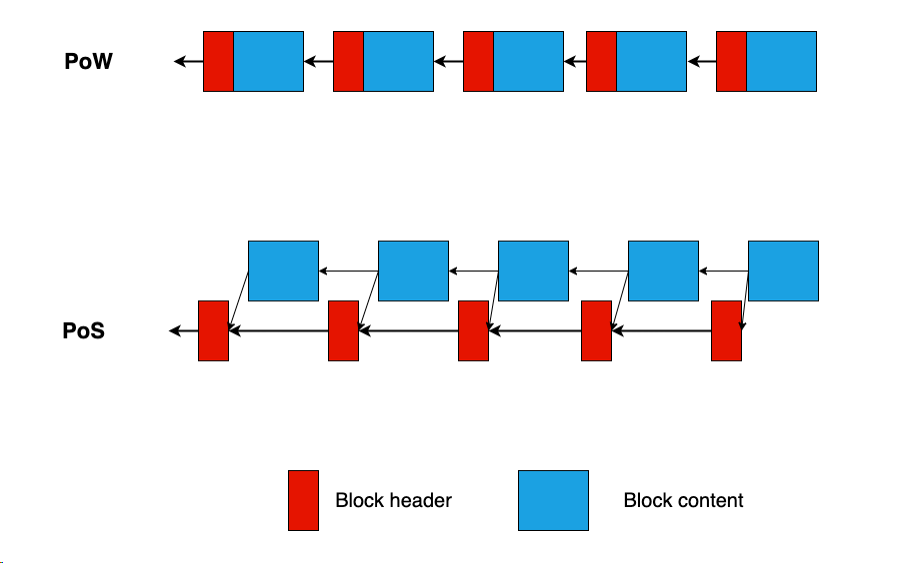
\includegraphics[width=0.7\linewidth]{Fig/11/F1}
    \caption{PoW vs. PoS}
    \label{fig:f1}
\end{figure}
The block headers are connected by hashes, but the block contents also have hashes that link them together (see Figure \ref{fig:f1}). This way, the attacker cannot change the whole chain if some blocks belong to honest nodes. However, an adaptive attacker can still take over all honest nodes that have blocks on the chain and then change any block they want. We can stop this by using a special technique called \textbf{Key Evolving Signature (KES)}.

\section{Key Evolving Signature (KES)}
Key-Evolving Signatures (KES) are used to sign blocks in a PoS mechanism. KES allows the block proposer to update their secret key in every step while keeping their public key the same. The old secret key is erased, so that it cannot be used to sign old blocks. This prevents an attacker from forging old signatures with new keys, and helps achieve adaptive security. Adaptive security means that the PoS mechanism can resist an attacker who tries to corrupt old blocks sometime in the future.\\\\
A simple example of KES involves periodically changing the secret key of any coin by its hash output. The block content has to be signed by the lottery winner with KES. We can make honest nodes delete all the old keys, which makes sure that the content of honest blocks cannot be changed by an adaptive attacker.

\subsection*{Verifiable Random Function (VRF)}
The public keys of the nodes are known to everyone, so the lottery winner is not a secret. This means that an attacker can try to harm or bribe a node that will win the lottery in the future. We can prevent this by using a special technique called \textbf{verifiable random function (VRF)}\\\\
VRF is a function that takes a secret key and an input, and produces an output and a proof. The output is random and unpredictable, but anyone can verify that it was generated by the secret key and the input, using the public key and the proof.
\thm{VRF}{\begin{align}
        VRF( sk , x ) \rightarrow ( y , \pi )
\end{align}  The secret key $sk$ and the input $x$ are used to generate the output $y$ and the proof $\pi$
\begin{align}
    Verify( pk , x , y , \pi ) \rightarrow True/False
\end{align}  The public key $pk$, the input $x$, the output $y$, and the proof $\pi$ are used to check if the output is valid or not.}
\dfn{POS idea 4}{A node n succeeds in mining a block if \begin{align}
        \label{eq:7}
        VRF(hash(parent.header), ts, sk_n) < T \times stake_n
\end{align}}
VRF makes the block proposer selection more random and secret, so that the attacker cannot predict or influence who will win the lottery. VRF is therefore a powerful tool for enhancing the security and fairness of the PoS mechanism.

\section{Nothing at Stake attack}
The honest participants follow the longest chain rule, which means they only mine on the end of the longest chain. The attacker, however, mines on many places in the chain tree, and tries to create a longer chain than the honest one. The attacker can do this because they can use the same stake to mine many blocks without spending much resources. 
\begin{figure}[h!]
    \centering
    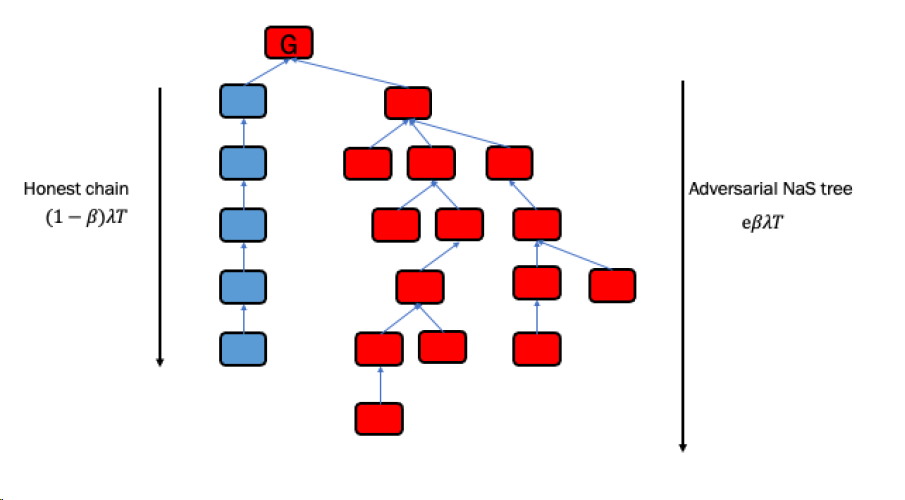
\includegraphics[width=0.7\linewidth]{Fig/11/F2}
    \caption{NaS attack}
    \label{fig:f2}
\end{figure}\\
The honest chain grows linearly in time, like a Poisson process, with a rate of $(1 - \beta)\lambda T$, while the attacker’s chain grows exponentially in time, as a NaS tree, with a length of $e\beta\lambda T$, where $e$ is the base of the natural logarithm. NaS attack allows the attacker to compete with the honest participants unevenly, as they can cheat and manipulate the chain.
The effect of the NaS attack is to amplify the growth rate of the private chain by a factor of $e$. \\\\
The NaS attack is successful when 
\begin{align}
    (1 - \beta)\lambda T > e\beta\lambda T \quad \Rightarrow \quad \beta <\frac{1}{1+e}\cong27\%
\end{align}
We have seen a balancing attack on GHOST, which can work with less than 50\% of the hash power. Can we do something similar with PoS? The answer is no, because the private attack is the worst-case scenario for PoS. The protocol can resist any attack as long as $\beta < \frac{1}{1+e}$. This means that the attacker’s stake must be less than 27\% of the total stake. This is the exact security threshold for this protocol. It is about half of the security threshold for PoW, which is 50\% of the hash power.

\section{Boosting Security Threshold}
We might wonder if we can make the threshold 50\%, like in PoW's longest chain. We want to do this with a simple change in the PoS protocol. We notice that the previous PoS protocol is weak to the NaS attack because each block in the chain tree gives a new random source and starts a new lottery. We can fix this by changing the random source less often.
\dfn{Ouroboros PoS}{A first-order idea is to never update the randomness and only draw it
    from the genesis block.}
The Ouroboros PoS protocol proceeds in discrete epochs; essentially a new genesis block starts off each epoch.
\dfn{POS idea 5}{A node n succeeds in mining a block if \begin{align}
        \label{eq:9}
        VRF(hash(Genesis), ts, sk_n) < T \times stake_n
\end{align}}
Some recent studies have shown that the protocol in Equation 6 is safe if most of the stake is honest, which is the same as the PoW longest chain protocol. They also showed that the private attack is the hardest attack to stop, and the security threshold (on honest stake) is the best one. They used the same proof method of Nakamoto blocks that we used for the NaS attack.\\\\
The adversary can also try to bribe some of the block proposers in the Ouroboros Praos protocol by setting up a website that offers rewards for their credentials in a future epoch (see Figure \ref{fig:f3}). This way, the adversary can learn who will be the next block proposers before anyone else (because of VRF) and use them to launch a deadly attack. \\
For example, the adversary can create a forked version of the blockchain with the help of the bribed proposers and keep it secret until a block s is confirmed by the k-deep rule. Then, the adversary can reveal the forked blockchain to everyone, making it the longest chain and replacing $s$ with $s′$ (which contains a double spend). Note that this attack only requires $k + 1$ out of $2k + 1$ lotteries to be won by the bribed proposers, who may have a very small stake in total.
\begin{figure}[h!]
    \centering
    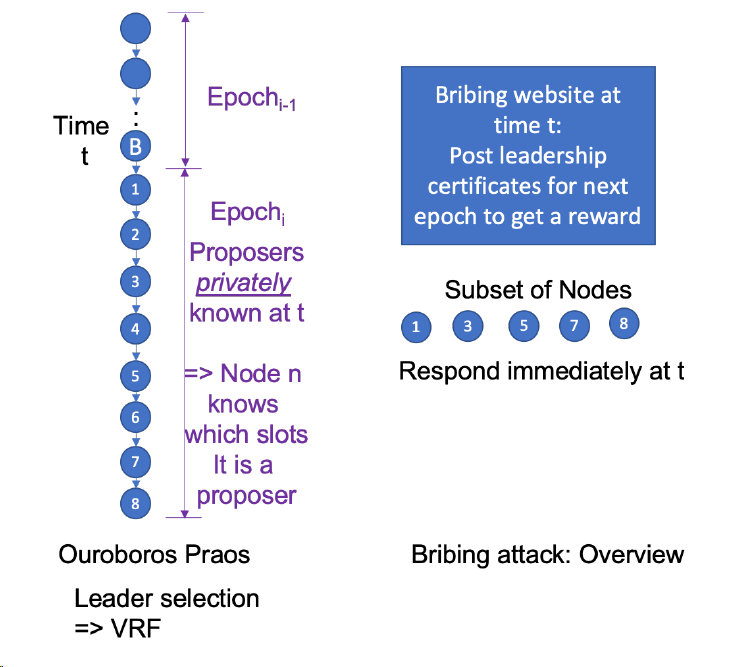
\includegraphics[width=0.55\linewidth]{Fig/11/F3}
    \caption{Structure of bribing attack}
    \label{fig:f3}
\end{figure}
\begin{figure}[h!]
    \centering
    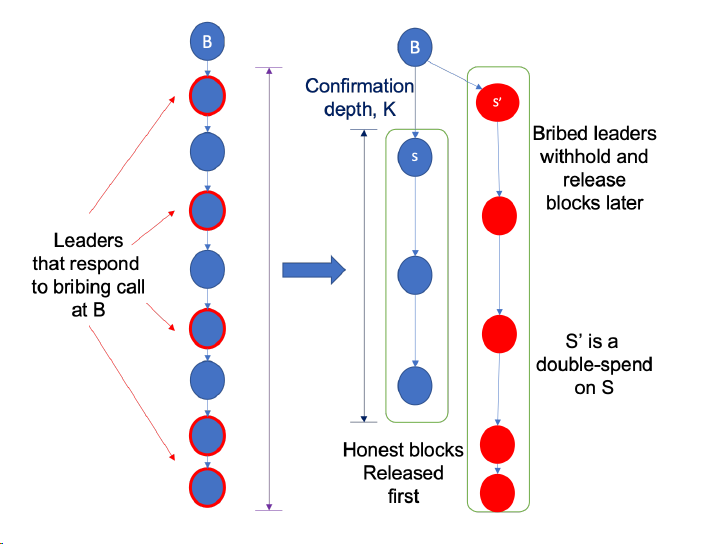
\includegraphics[width=0.55\linewidth]{Fig/11/F4}
    \caption{Bribing attack on Ouroboros Praos}
    \label{fig:f4}
\end{figure}

\subsection{c-correlation PoS protocol}
The $c$-correlation property states that the updates of the randomness source are correlated with the multiples of a parameter $c$, which controls the security level of the protocol. In this rule, the common source of randomness remains the same for $c$ blocks and is updated only when the current block to be generated is at a depth that is a multiple of $c$.
\begin{figure}[h!]
    \centering
    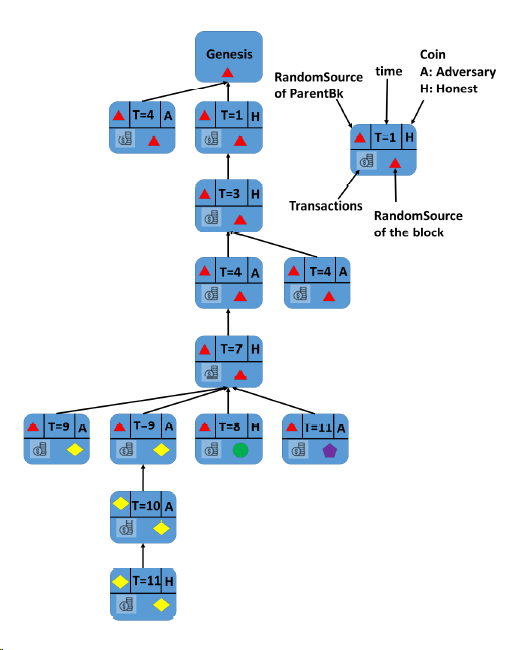
\includegraphics[width=0.5\linewidth]{Fig/11/F5}
    \caption{A snapshot of a block tree under c-correlation protocol with $c = 5$.}
    \label{fig:f5}
\end{figure}\\
When updating, the hash of the block header is used as the new source of randomness, i.e.,
\begin{align}
    \text{RandSource}(b) := \begin{cases}
        \text{VRF}(\text{RandSource}(\text{parent}(b)), ts, $sk$) \qquad\qquad & \text{ if } \text{depth}(b) \% c = 0\\
        \text{RandSource}(\text{parent}(b)) & O.W. 
    \end{cases}
\end{align}
\dfn{POS idea 5.2}{A node n succeeds in mining a block if \begin{align}
        VRF(\text{RandSource}(Genesis), ts, sk_n) < T \times stake_n
\end{align}}
The protocol in Equation (\ref{eq:7}) has the lowest value of $c$, which is $1$. This means that the randomness source updates with every block, but it also makes the NaS attack very easy. The protocol in Equation (\ref{eq:9}) has the highest value of c, which is $\infty$. This means that the randomness source updates only once per epoch, but it also makes the NaS attack impossible. By changing the value of c, we can adjust the security level of the protocol (see Table 1). Figure 6 shows that with c-correlation, we can achieve the same security as the current Ouroboros protocol used by Cardano, but with a much smaller epoch size.
\begin{figure}[h!]
    \centering
    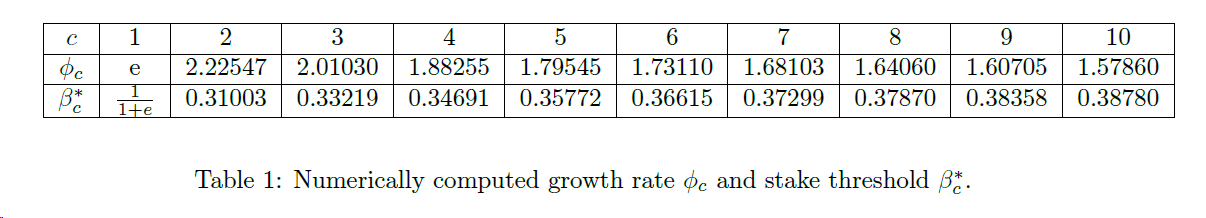
\includegraphics[width=\linewidth]{Fig/11/F6}
\end{figure}
\begin{figure}[h!]
    \centering
    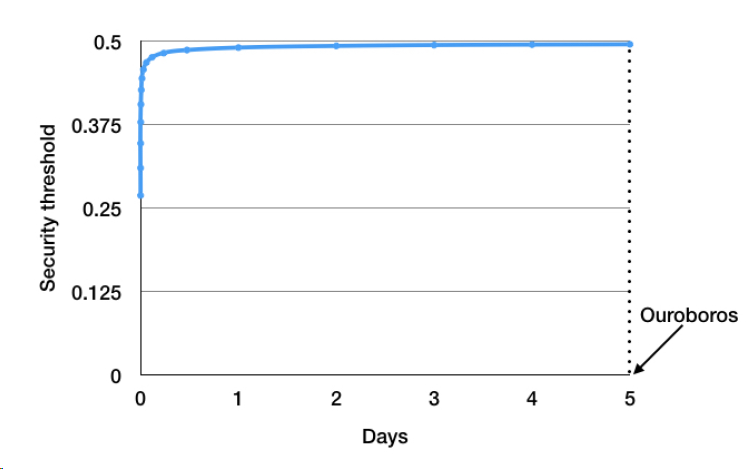
\includegraphics[width=0.5\linewidth]{Fig/11/F7}
    \caption{The security threshold $\beta_c^*$
        c of c-correlation against the epoch size, equaling to c times the
        inter-block time, which we set to be 20s, to match the implementation of Ouroboros in Cardano. The
        Cardano project currently updates the common randomness every 5 days (21600 blocks), while the
        security threshold of c-correlation can approach 1/2 with much higher randomness update frequency}
    \label{fig:f7}
\end{figure}

\section{Dynamic Stake}
So far the stake of the nodes that determines their success in the lottery is fixed, i.e., not changing. \\
This is bad for two reasons:
\begin{itemize}
    \item A node that has no stake now can still participate in the lottery (making it hard for new nodes to join)
    \item A node that has a lot of stake now cannot use its coins for anything else (making it easy for old nodes to dominate)
\end{itemize}
A better way is to let the dynamic stake of the nodes decide their success in the lottery; after all, the ledger is updated dynamically as new blocks are added to the longest chain and confirmed (when deep enough) and the security of the PoS longest chain rule ensures that all the honest nodes agree on the ledger.\\\\
The stake of a node n in the dynamic stake setting depends on both time and chain. Different chains in the blocktree have different transactions, which affect the stake of each node. We need to say which chain we are talking about when we look at the stake of a node. If we just use the state of the previous block to decide the stake of each node, the adversary can grind
on the stake of its coin.\\\\
The stake-grinding attack is when the adversary uses its stake to increase its chances of winning the next round. The adversary does this by creating two blocks with the same header, but different transactions. In one block, it moves its stake from one coin to another; in the other, it does the opposite. In the example of Figure 7, the adversary has coin A and coin B. When it can propose a block, it makes two blocks: one with A to B, and one with B to A. In the next round, the adversary can use both coins to play the lottery, so it has twice the chance of winning by changing its stake.

\begin{figure}[h!]
    \centering
    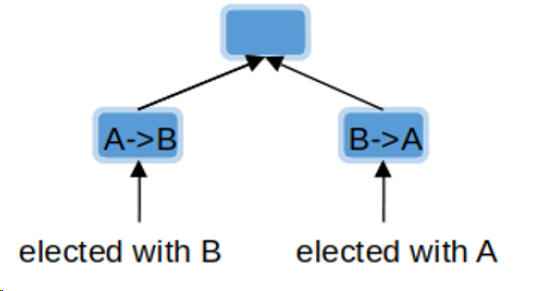
\includegraphics[width=0.3\linewidth]{Fig/11/F8}
    \caption{Stake grinding attack}
    \label{fig:f8}
\end{figure}

A simple way to stop the stake grinding attack is to use the stake in the block that is s blocks behind the current block on the main chain, where s is big enough so that everyone agrees on that block. But this still has a problem. Imagine the adversary making its own secret chain from the start (or any block in the blocktree). At first, the secret chain grows at a speed of $\beta\lambda$. But after s blocks from the start of the secret chain, the adversary can start changing the private key of its coin; when it finds a good coin, it can move its stake to that coin by adding transactions in the first block in the secret chain. This is possible because all the blocks in the secret chain are made by the adversary. It can change anything in the secret chain and sign all the previous blocks again.\\\\
The adversary can use this stake-grinding attack to win the lottery every time in the secret chain, and eventually catch up with the public block tree, which grows at a fixed speed $(1 - \beta)\lambda$. To stop this attack, we suggest a new way to choose between forks called s-truncated longest chain.

\subsection{New fork choice rule}
The stake-grinding attack makes the private chain grow slowly at first, so we cannot just compare the length of the chains when they split. We need a different way to choose the best chain. We use the s-truncation rule, which compares the density of the chains after the fork. The density is how many blocks are in the first s blocks after the fork. The honest node always has one main chain that it adds its new block to. When it gets a new chain of blocks, it has to decide which chain to keep. It does not look at the length of the two chains, like in the longest chain rule. It looks at the time it took to make the first s blocks after the fork in both chains. The chain that is faster and denser is the better chain.\\\\
The block where the two chains diverge is $b_{fork}$. The honest node compares how much time each chain takes to produce s blocks after $b_{fork}$. The chain that is faster and denser is the better chain. The honest node will attach its new block to the last block of that chain.\\\\
We have one more thing to say about the s-truncation rule. We only use it when we compare two chains that both have s or more blocks after they split. If one of the chains has less than s blocks after the split, we use the longest chain rule to choose the best chain. This is how we make the PoS lottery work well, even when the stake changes over time.

\section{Dynamic Availability Using VDF}
Bitcoin has a nice feature called dynamic availability: Bitcoin can deal with a changing and unknown level of mining power; Miners can come and go as they wish without any sign-up process. Is it possible to have the same feature in the PoS version?\\\\
The protocol we have shown so far works well if only a small part (for example, 27\% for c = 1) of the online nodes are adversarial, but it also needs another thing: all the bad nodes are always online. This might seem fair (why would a bad node go offline?), but in real life this can be very hard. Usually, in public blockchains, PoW or PoS, no node is bad at the start of a new blockchain token (because the token is not worth much); bad nodes only show up later on.\\\\
The protocol needs another thing to work well: all the bad nodes are always online. This is not just extra, but very important for the security. Imagine that in the first year of the PoS blockchain, only 10\% of the stake is online. All of them are good nodes. Then, in the second year, all 100\% of the stake is online, but 20\% is bad. Even though most of the online stake is good, the protocol is not safe because the bad nodes can use their 20\% stake to go back in time and win all the past blocks from the start. Then they can make a chain very fast from the start and make it longer than the current chain (see Figure \ref{fig:f9}(a)). This is possible because making blocks in the PoS protocol is very cheap (just need to play all the old lotteries). So, when bad nodes come online, they can change not only the present, but also the past. PoW does not have this problem because it takes a lot of time and work to make a chain from the past and that chain will always be shorter than the current chain. So, PoW has a sense of time, which means nodes cannot change the past blocks when they are offline. This is why PoW can handle dynamic nodes, where both good and bad nodes can come and go (see Figure \ref{fig:f9}(b)).
\begin{figure}[h!]
    \centering
    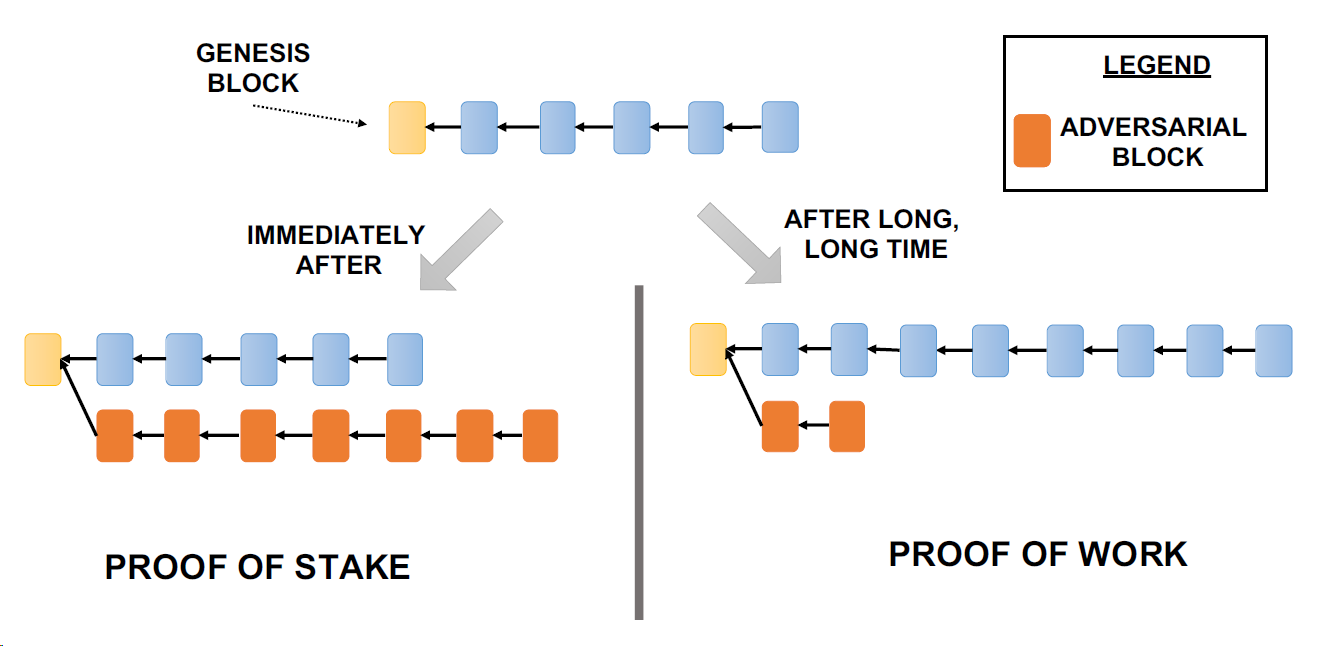
\includegraphics[width=0.7\linewidth]{Fig/11/F9}
    \caption{(a) Newly coming online stakeholders in the PoS protocol can grow a chain from genesis
        instantaneously. (b) Newly joined miners in the PoW protocol take a long time to grow such a chain
        and are always behind.}
    \label{fig:f9}
\end{figure}
\subsection{PoSAT}
PoSAT is a new idea that solves the problem of dynamic nodes in PoS. It uses a special kind of function called \textbf{Verifiable Delay Function (VDF)} to make the block lottery depend on time. VDFs are built on top of iteratively sequential functions, i.e., functions that are only computable sequentially: $f^l(x) = f \circ f \circ ... \circ f(x)$/, along with the ability to provide a short
and easily verifiable proof that the computed output is correct.\\\\
Examples of such functions include (repeated) squaring in a finite group of unknown order, i.e., $f(x) = 2^x$ and (repeated) application of secure hash function (SHA-256), i.e., $f(x) = Hash(x)$.\\
The VDF also gives proof for each answer, and the proof can be checked quickly. This is amazing! VDFs can show how much time has passed (if we know how fast the CPU is), and they can also make random numbers. So, we can use VDF to run the lottery until a random time $L$ when $f^L(x)$ is small enough. Then $L$ will be a random number with a certain shape. This VDF lottery can create a sense of time in PoS.
\dfnc{PoS idea 6}{A node n succeeds in mining a block if \begin{align}
        VDF(\text{RandSource}(parent), ts, sk_n) < T \times stake_n
\end{align}}
With VDF, the adversary cannot go back in time and create a longer chain than the honest
chain immediately, because creating a longer chain now requires time. While the adversarial chain is
growing, the honest chain is growing at a larger speed. Therefore, PoSAT is secure in the dynamic
available setting.